\documentclass[../handbook.tex]{subfiles}
\graphicspath{{\subfix{../pics/}}}
\begin{document}

\section{Cookbook}

\begin{enumerate}
    \item \emph{Репозиторий.} Анализ самостоятельного датасета лучше поместить
        в отдельную папку.

    \item \emph{Описальные статистики} стоит просмотреть чтобы понять качество
        данных и исключить сильные аномалии.

    \item Построить \emph{гистограмму} чтобы понять распределение и проверить
        на выбросы.\marginpar{Иногда удобно просматривать логарифмированную
        фичу. Если фича сильно отстоит от нуля, ее лучше переместить в ноль.}

\end{enumerate}

\section{Train, Test, Validation}
\begin{marginfigure}
    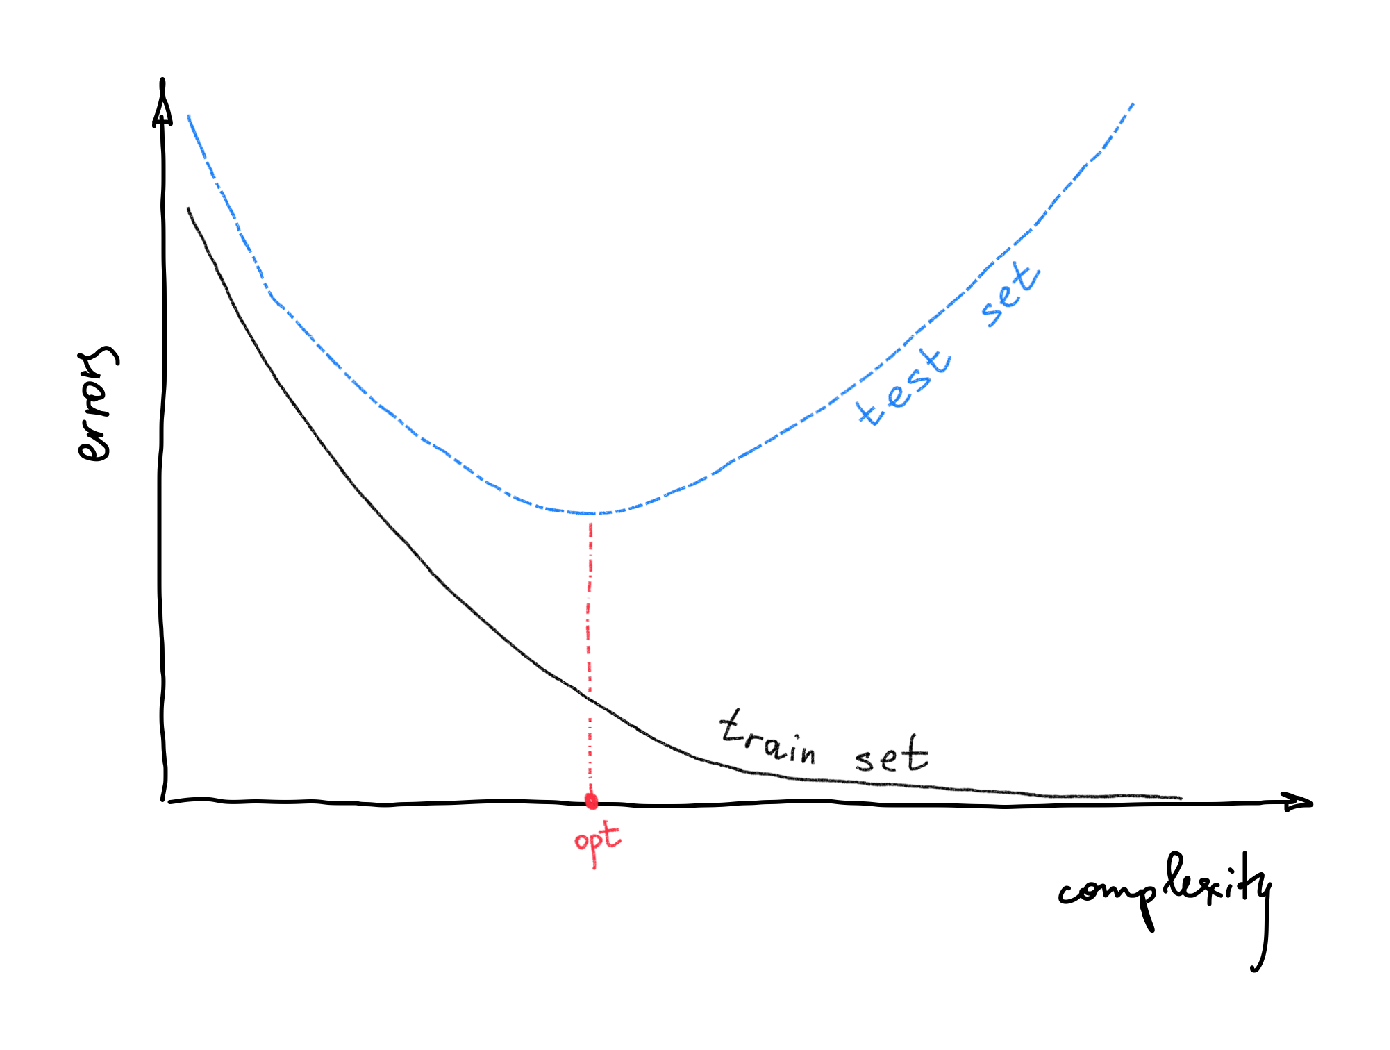
\includegraphics[width=1\columnwidth]{pics/choise_of_model.pdf}
    \caption{\emph{Выбор модели:} по оси абсцисс лежат модели (например, это могут быть степени аппроксимирующих многочленов), по оси ординат отмечается ошибка. Выбирается та модель у которой достигается наименьшая ошибка на тестовой выборке (на рисунке точка opt).}
    \label{fig:choise_of_model}
\end{marginfigure}
Общая рекомендация относить в тестовую выборку до 30\% всех данных. Методику с train-test'ом используют чтобы выбрать модель которой. Например, в задаче регрессии нужно понять многочленами какой степени стоит аппроксимировать данные. Отбирается та модель которая на тестовой выборке показывает минимальную ошибку. В цлеом это так или иначе упирается в кросс-валидацию.

\begin{itemize}
    \setlength\itemsep{0em}
    \item Обучащающая выборка - для обучения модели
    \item Тестовая выборка - для замера качества модели
    \item Валидационная выборка - для подбора гиппер-параметров
\end{itemize}

Альтернативой к валидации является подход с регуляризацией.

\end{document}
